\begin{figure}[t!]
\centering
\resizebox{\textwidth}{!}{%
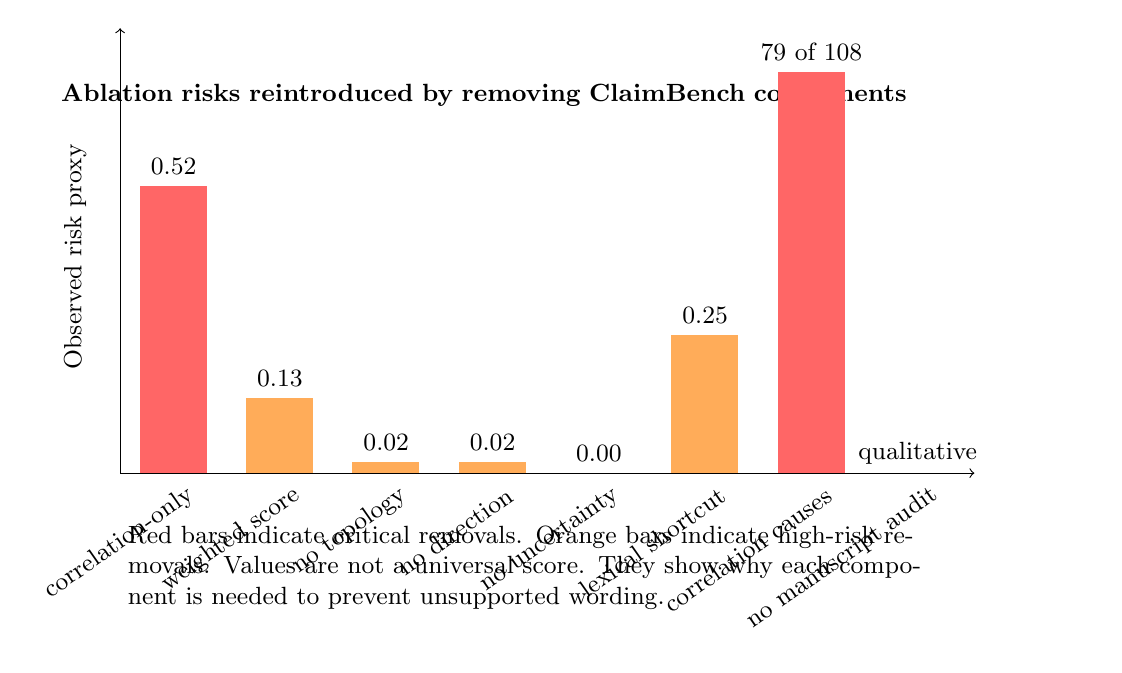
\begin{tikzpicture}[font=\small]
\node[align=left, text width=13cm] at (5.5,4.8) {\textbf{Ablation risks reintroduced by removing ClaimBench components}};
\foreach \x/\h/\lab/\val/\col in {
0/3.65/correlation-only/0.52/red!60,
1.35/0.95/weighted score/0.13/orange!65,
2.7/0.14/no topology/0.02/orange!65,
4.05/0.14/no direction/0.02/orange!65,
5.4/0.0/no uncertainty/0.00/gray!60,
6.75/1.75/lexical shortcut/0.25/orange!65,
8.1/5.1/correlation causes/79 of 108/red!60,
9.45/0.0/no manuscript audit/qualitative/orange!65}
{
  \fill[\col] (\x,0) rectangle +(0.85,\h);
  \node[rotate=35, anchor=east] at (\x+0.75,-0.18) {\lab};
  \node at (\x+0.43,\h+0.25) {\val};
}
\draw[->] (-0.25,0) -- (10.6,0);
\draw[->] (-0.25,0) -- (-0.25,5.65);
\node[rotate=90] at (-0.82,2.75) {Observed risk proxy};
\node[align=left, text width=10.5cm] at (5.1,-1.2) {
Red bars indicate critical removals. Orange bars indicate high-risk removals. Values are not a universal score. They show why each component is needed to prevent unsupported wording.
};
\end{tikzpicture}%
}
\caption{Component ablation summary. Removing non-compensatory gating, causal abstention, or evidence separation reintroduces overclaiming risks that would be hidden by ordinary predictive evaluation.}
\label{fig:ablation}
\end{figure}
